\begin{frame}{Reformulate the Problem-\only<1>{A}\only<2>{B}}
  \begin{minipage}{0.5\textwidth}
\only<1>
{
    \begin{block}{\color{White} $\mathbf{P}=\mathcal{C}(\mathbf{F})$}
      \begin{itemize}
        \item Normally, $\mathbf{P}=f(\mathbf{F}, \boldsymbol\gamma)$
        \item $\boldsymbol{\gamma}:=\{\gamma_i\}_{i=1}^{M}$ with $M\in\mathbb{Z}^+$
        \item $\mathbf{P}=\mathcal{M}(\mathbf{F}, \boldsymbol{\gamma})$
        \item Application specific models! 
      \end{itemize}
    \end{block} 
}
\only<2>
{
    \begin{block}{\color{White} $\mathbf{P}=\mathcal{C}(\mathbf{F})$}
      \begin{itemize}
        \item Let's stick to $\mathbf{P}=\mathcal{C}(\mathbf{F})$
        \item Then, $\mathbf{P}=\mathcal{M}(\mathbf{F})$
      \end{itemize}
    \end{block} 
    \begin{block}{\color{White} How to account for $\boldsymbol{\gamma}$?}
      \begin{itemize}
        \item Let's stick to $\{\mathbf{P}_i=\mathcal{C}_i(\mathbf{F})\}_{i=1}^{M}$ with $M\in\mathbb{Z}^+$
        \item $\mathbf{P}=\mathcal{M}(\mathbf{F})$
        \item Model input-output remains the same!
      \end{itemize}
    \end{block} 
}
  \end{minipage}%
  \begin{minipage}{0.5\textwidth}
    \centering
    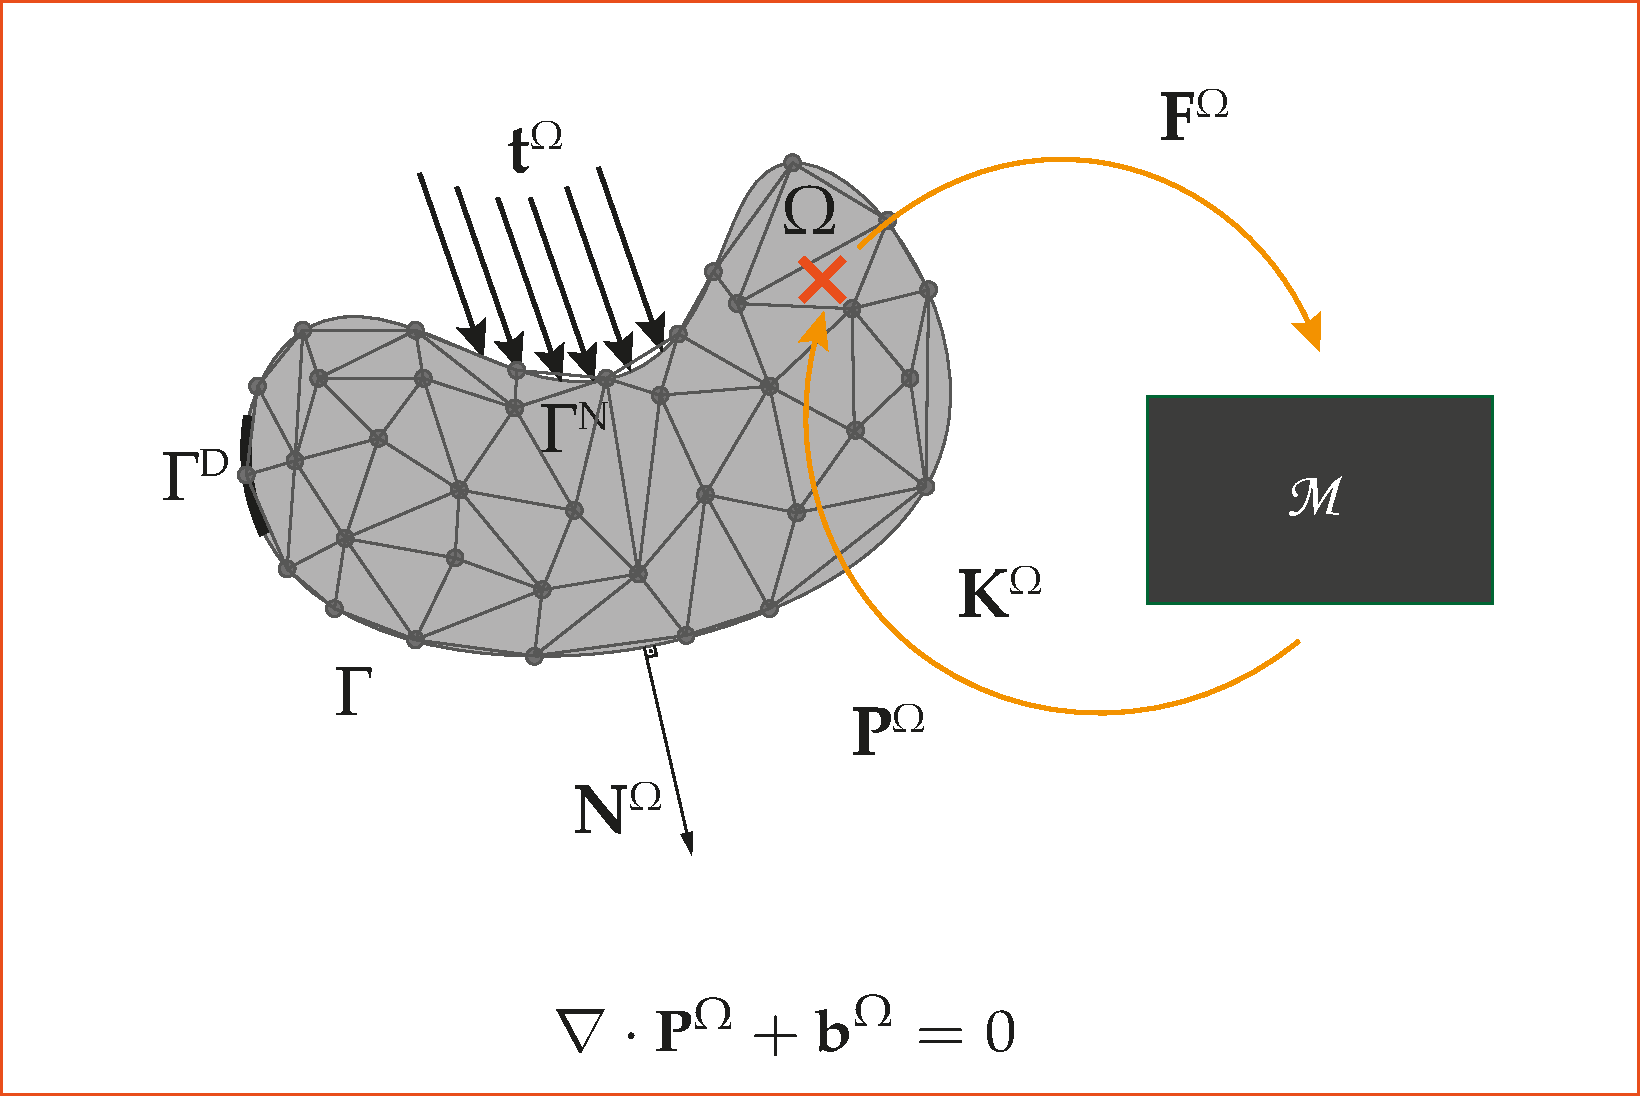
\includegraphics[width=0.9\textwidth]{Figures/literature/FE2-ML.pdf} 
  \end{minipage}
\end{frame}

\begin{frame}{Reformulate the Problem-\only<1>{C}\only<2>{D}}
  \begin{minipage}{0.5\textwidth}
\only<1>
{
    \begin{block}{\color{White} How do we end up with a parametrized relationships?}
      \begin{itemize}
        \item Series of assumptions, $\mathcal{A}:\{a_n \subset a_{n-1} \subset ... \subset a_1\}$ 
     \end{itemize}
    \end{block} 
    \begin{block}{\color{White} Individual Learning Problem}
      \begin{itemize}
        \item If the aim is to learn $\mathbf{F} \to \mathbf{P}$ 
        \item Learning problem: $\mathcal{T}_\mathcal{A}:\mathbf{F} \to \mathbf{P}$
      \end{itemize}
    \end{block}
}
\only<2>
{
    \begin{block}{\color{White} Overall Learning Problem}
      \begin{itemize}
        \item Given $\{\mathbf{P}_i=\mathcal{C}_i(\mathbf{F})\}_{i=1}^{M}$ with $M\in\mathbb{Z}^+$
        \item Learning problem: $\{\mathcal{T}_{\mathcal{A}_i}:\mathbf{F} \to \mathbf{P}_i\}_{i=1}^{M}$
      \end{itemize}
    \end{block} 
}
  \end{minipage}%
  \begin{minipage}{0.5\textwidth}
    \centering
    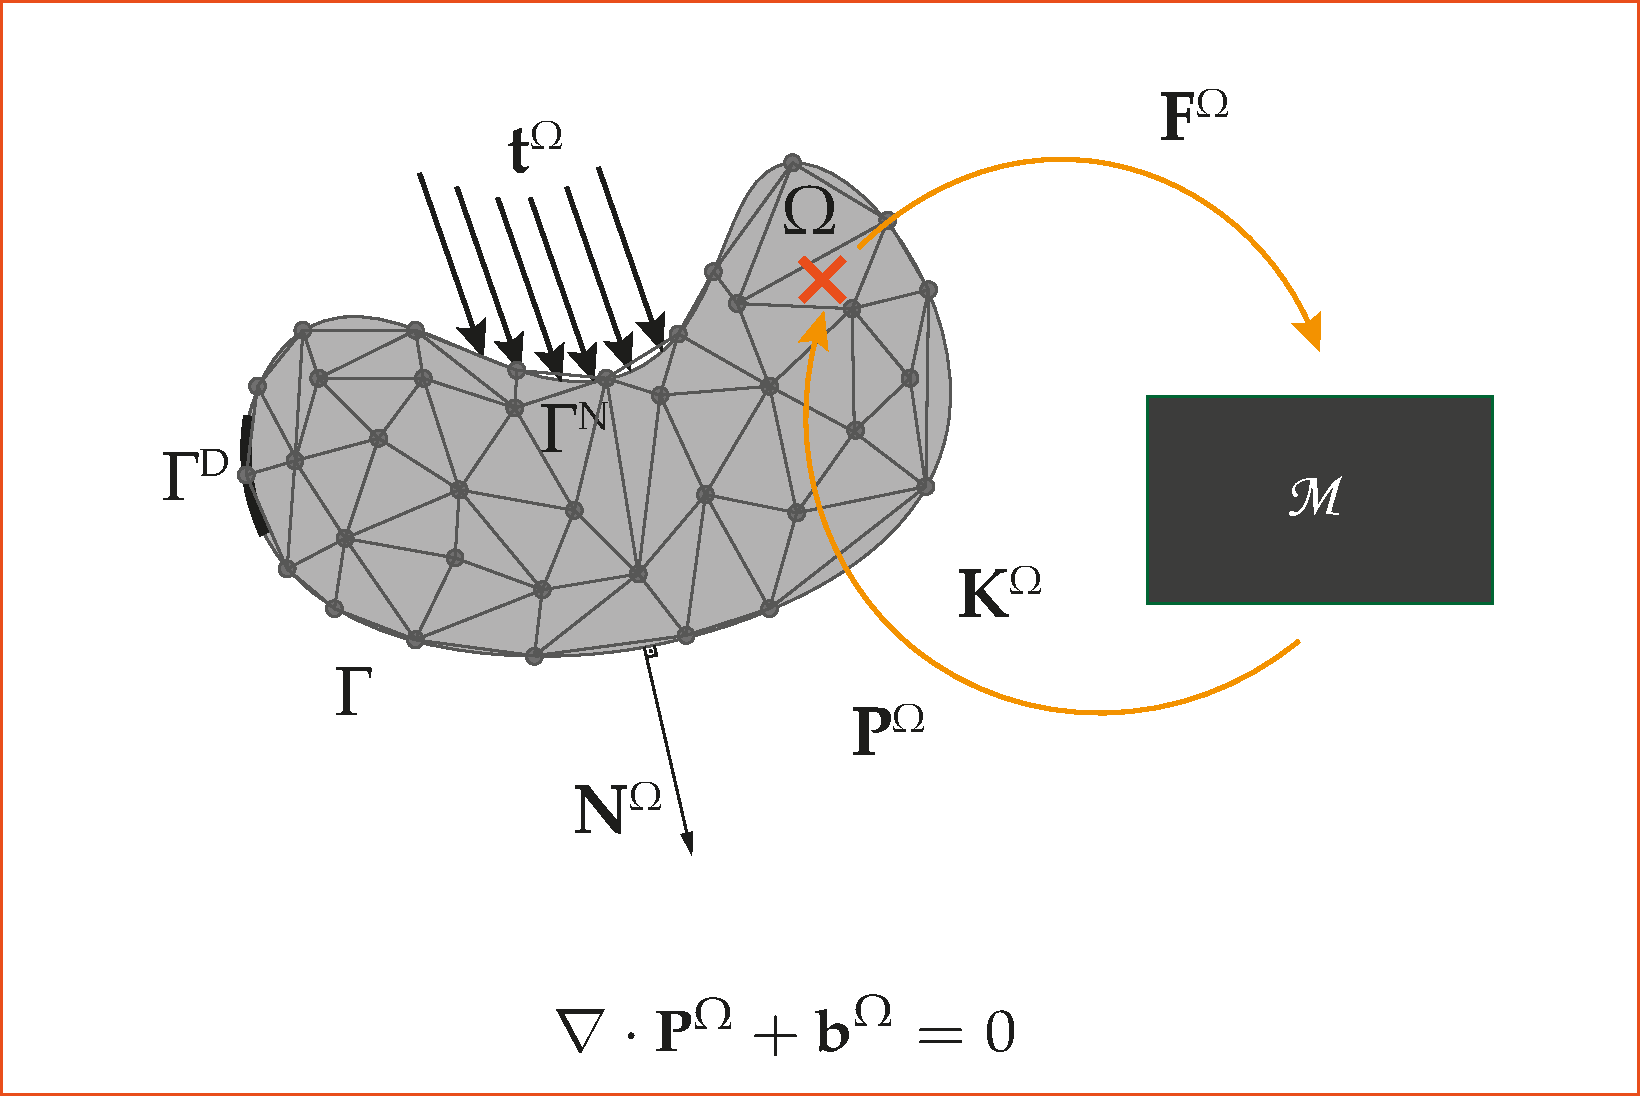
\includegraphics[width=0.9\textwidth]{Figures/literature/FE2-ML.pdf} 
  \end{minipage}
\end{frame}

\begin{frame}{Single-Task Learning vs Bias Learning-\only<1>{A}\only<2>{B}}
  \only<1>
  {
    \begin{block}{\color{White} Single-Task Learning}
      \begin{itemize}
        \item Input Space $\mathbf{F}$ OutputSpace $\mathbf{P}$
        \item Probability Distribution $p$ on $\mathbf{F}\times\mathbf{P}$
        \item Loss Function $l:\mathbf{P}\times\mathbf{P}\to \mathbb{R}$
        \item Hypothesis Space $\mathcal{H}$, a set of functions $h:\mathbf{F}\to\mathbf{P}$
        \item Minimize the expected loss to get $h\in\mathcal{H}$
      \end{itemize}
    \end{block}
  }
  \only<2>
  {
    \begin{block}{\color{White} Bias  Learning}
      \begin{itemize}
         \item Input Space $\mathbf{F}$ OutputSpace $\mathbf{P}$
        \item Probability Distribution $p$ on $\mathbf{F}\times\mathbf{P}$
        \item Loss Function $l:\mathbf{P}\times\mathbf{P}\to \mathbb{R}$
        \item An environment $(\mathcal{Q},\mathcal{P})$ where $\mathcal{P}$ is all possible distribution of $p$ and $\mathcal{Q}$ is the distribution of $\mathcal{P}$
        \item Hypothesis Space Family $\mathbb{H}:=\{\mathcal{H}\}$, where each $\mathcal{H}$ is a set of functions $h:\mathbf{F}\to\mathbf{P}$
        \item Minimize the expected future risk or transfer risk to find the appropriate Hypothesis Space $\mathcal{H}$ 
      \end{itemize}
    \end{block}
  }
\end{frame}

\begin{frame}{MAML vs Multi-task}
	\begin{itemize}
		\item Problem: $y=a*\text{sin}(x+p)$ for $x\in[0,5]$ and $a\in[0.1,5]$ \& $a\in[0,\pi]$ for $\text{K}=5$ and $\mathcal{B}(\mathcal{T})$ size $100$
	\end{itemize}
	\begin{minipage}{0.5\textwidth}
		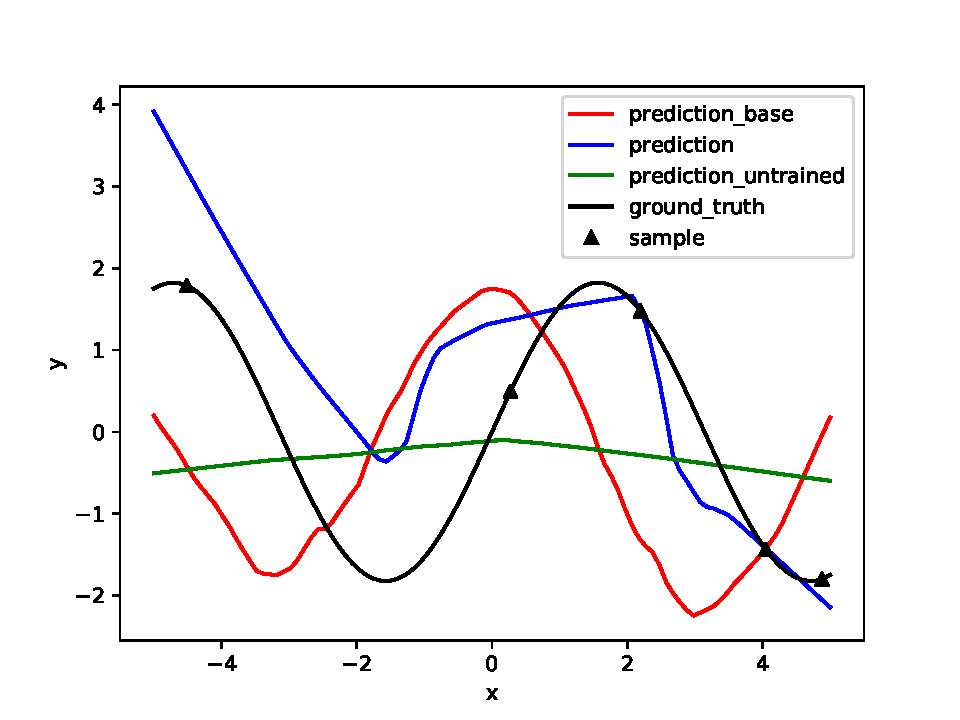
\includegraphics[width=0.9\textwidth]{Figures/Study1/sine-hard-finn-maml-pred.pdf}
		\centering
			MAML
	\end{minipage}%
	\begin{minipage}{0.5\textwidth}
		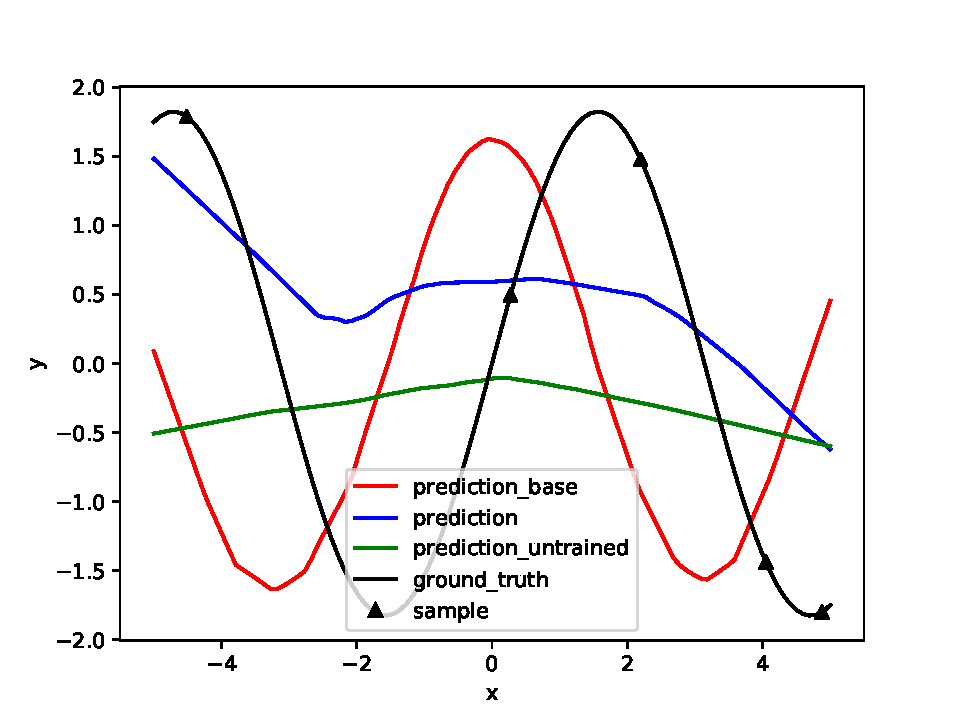
\includegraphics[width=0.9\textwidth]{Figures/Study1/sine-hard-finn-multitask-pred.pdf}
		\centering
			Multi-task
	\end{minipage}
\end{frame}

\begin{frame}{Small Investigation of MAML \cite{Finn2017}}
  \begin{minipage}{0.5\textwidth}
    \begin{itemize}
      \item $ a \in \mathbb{R}^d \to p_a \sim \mathcal{N}(m\mathbf{1},c\mathbf{I})$
      \item $ x \in \mathbb{R}^d \to p_x \sim \mathcal{U}(\mathbf{0},b\mathbf{1})$
      \item $ \varepsilon \sim \mathcal{N}(0,\sigma^2)$
      \item $ y = a^\text{T}x + \varepsilon \quad \in \mathbb{R}$
      \item $ Z:= ((x_i,y_i))_{i=1}^N$
      \item $ \hat{a}_N \to $ an estimator trained with N training points
    \end{itemize}
  \end{minipage}%
  \begin{minipage}{0.5\textwidth}
    Expected Error over the whole task space,
      $ \int \int \int (\hat{a}_N(Z)^{\text{T}}x-y)^2p(x,y)dxdyp_ZdZp_ada$
  \end{minipage}
  \color{Pink} Investigating the performance of a future emprical risk minimizing algorithm for transfer risk.
\end{frame}

\begin{frame}{F3DASM}
\centering
\begin{minipage}{0.55\textwidth}
		\begin{itemize}
		\item Design of Experiements
		\item Simulation or Machine Learning Module
	\end{itemize}	
\end{minipage}

\begin{minipage}{0.4\textwidth}
	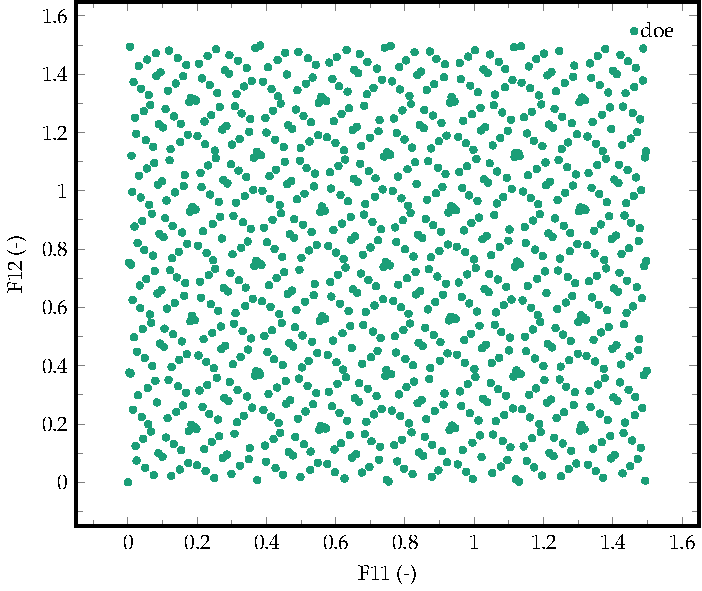
\includegraphics[width=\textwidth]{Figures/F3DASM/doe}
\end{minipage}%
\hspace{1mm}$\xRightarrow{\text{FEM}(\mathbf{F})}$
\begin{minipage}{0.4\textwidth}
	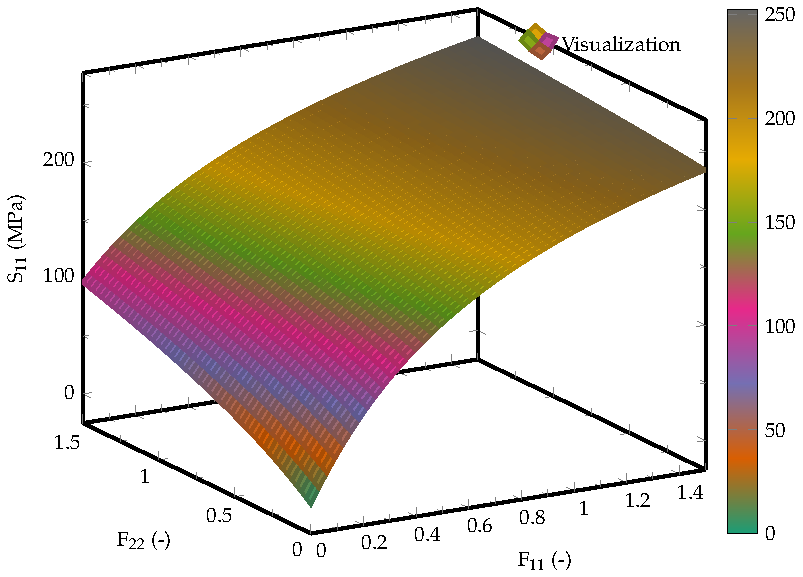
\includegraphics[width=\textwidth]{Figures/F3DASM/manifold}
\end{minipage}%
\end{frame}

\begin{frame}{Summer Schools \& Conferences}
\only<1>
{
  \begin{block}{\color{White} Summer Schools}
  \begin{itemize}
    \item Machine Learning Summer Schools (MLSS)
    \item Gaussian Process Summer School 
    \item Nordic Probabilistic AI Summer School
    \item Oxford Machine Learning Summer School
  \end{itemize}
  \end{block}
}
\only<2>
{
  \begin{block}{\color{White} Conferences on ML}
  \begin{itemize}
    \item Conference on Computer Vision and Pattern Recognition (CVPR)
    \item International Conference on Learning Representations (ICLR)
    \item International Conference on Machine Learning (ICML)
    \item International Conference on Machine Learning and Pattern Recognition (ICMLPR)
  \end{itemize}
  \end{block}
}

\only<3>
{
  \begin{block}{\color{White} Conferences on Mechanics}
  \begin{itemize}
    \item FEniCS Conference
    \item International Conference on Mathematics and Computational Mechanics (ICMCM)
    \item International Conference on Computational Geomechanics and Material Response (ICCGMR)
    \item FEniCS Conference
    \item International Conference on Computational Continuum Mechanics and Dynamics (ICCCMD)
\item International Conference on Computational Continuum and Continuum Mechanics (ICCCM)
  \end{itemize}
  \end{block}
}
\end{frame}



